%!TeX spellcheck = en-UK

\documentclass{tufte-handout}

\title{Pre-Proposal for a Capstone Project Intended to Satisfy the Requirements for an ALM in Digital Media Design at Harvard Extension School}

\author[Dave Morgan]{Dave Morgan}

%\date{28 March 2010} % without \date command, current date is supplied

%\usepackage{geometry}
% \geometry{showframe} % display margins for debugging page layout

\usepackage{graphicx} % allow embedded images
\setkeys{Gin}{width=\linewidth,totalheight=\textheight,keepaspectratio}
\graphicspath{{graphics/}} % set of paths to search for images
\usepackage{amsmath}  % extended mathematics
\usepackage{booktabs} % book-quality tables
\usepackage{units}    % non-stacked fractions and better unit spacing
\usepackage{multicol} % multiple column layout facilities
\usepackage{lipsum}   % filler text
\usepackage{fancyvrb} % extended verbatim environments
\fvset{fontsize=\normalsize}% default font size for fancy-verbatim environments




% Standardize command font styles and environments
\newcommand{\doccmd}[1]{\texttt{\textbackslash#1}}% command name -- adds backslash automatically
\newcommand{\docopt}[1]{\ensuremath{\langle}\textrm{\textit{#1}}\ensuremath{\rangle}}% optional command argument
\newcommand{\docarg}[1]{\textrm{\textit{#1}}}% (required) command argument
\newcommand{\docenv}[1]{\textsf{#1}}% environment name
\newcommand{\docpkg}[1]{\texttt{#1}}% package name
\newcommand{\doccls}[1]{\texttt{#1}}% document class name
\newcommand{\docclsopt}[1]{\texttt{#1}}% document class option name
\newenvironment{docspec}{\begin{quote}\noindent}{\end{quote}}% command specification environment

% my packages
\usepackage{ amssymb } % for \checkmark
% counter for resuming enumerated list numbers
\newcounter{resumeenumi}
\newcommand{\suspend}{\setcounter{resumeenumi}{\theenumi}}
\newcommand{\resume}{\setcounter{enumi}{\theresumeenumi}}

\newcommand\lb{\linebreak}
\newcommand\pars{\par\smallskip}
\newcommand\parm{\par\medskip}
\newcommand\parb{\par\bigskip}

%left flushed minipage
\newcommand{\minit}[2][0.8]{
	\begin{minipage}[t]{#1\columnwidth}
		\raggedright
		#2
	\end{minipage}
}

%left flushed minipage
\newcommand{\mini}[2][0.8]{
	\begin{minipage}[c]{#1\columnwidth}
		\raggedright
		#2
	\end{minipage}
}



% centered minipage with text \raggedright
%\cmini[width]{content}
\newcommand{\cmini}[2][0.8]{
	\begin{center}
		\begin{minipage}{#1\columnwidth}
			\raggedright
			#2
		\end{minipage}
	\end{center}
}

% get x and y coordinates from a tikz coordinate
%\gettikzxy{A}{\ax}{\ay}
\makeatletter
\providecommand{\gettikzxy}[3]{%
	\tikz@scan@one@point\pgfutil@firstofone#1\relax
	\edef#2{\the\pgf@x}%
	\edef#3{\the\pgf@y}%
}
\makeatother




\begin{document}

\raggedright
\maketitle% this prints the handout title, author, and date

% \begin{abstract}
% 	% \noindent
% 	This document is a pre-proposal for Dave Morgan's capstone project, intended to satisfy requirements for an ALM in Digital Media Design at Harvard Extension School. The proposed project will involve the refactoring of a website authored a decade or so ago, and visible at \url{http://qwizm.org}.
% 	\parm\noindent
% 	Qwizm contains a number of quizzes or assignments, each comprised of questions having multiple parts. Input values to these questions are pseudo-randomized, and derived from a student ID number so that each student receives 'unique' question inputs. Answers are numerical.  To date, these questions have focused on problems in introductory engineering courses.
% 	\parm\noindent
% 	The aim of this refactoring is to make the site more accessible and user-friendly, and to take advantage of recent advances in technology allowed by HTML$5$, CSS$3$ and ES$6$. The proposed site will make it more convenient for instructors to create new questions and quizzes of their own and more convenient for students to use.
%
% \end{abstract}


\section{\Large Candidate Information}\label{sec:candidate}
\emph{First Name}: Dave \parm
\emph{Last Name}: Morgan \parm
\emph{ID}: 10823943 \parm
\emph{Education}: \\
\hspace{0.5cm}BSc. Applied Mathematics (2003), \\
\hspace{0.5cm}University of Calgary, Calgary, Alberta, Canada \parm
\hspace{0.5cm}BSc. Computer Science (2003), \\
\hspace{0.5cm}University of Calgary, Calgary, Alberta, Canada \parm
\emph{Current Employment}: Retired \parm
\emph{5-Year Deadline}: May, 2020 \parb

\section{\Large Capstone Track}
	ALM in Digital Media Design: Web Development

\section{\Large Courses Related to Capstone}\label{sec:project}
\begin{enumerate}
  \item Intensive Introduction to Computer Science (CSCI E-52)
	\item Developing Interactive Media (DGMD E-20)
  \item Web Programming/ JavaScript (CSCI E-3)
  \item Mobile Front-End Design II (DGMD E-27)
  \item Applied Online Course Design (DGMD E-60)
\end{enumerate}

\section{\Large Title and Brief Description}
\begin{itemize}
	\item Qwizm
	\item A client-side online testing system, for multiple-part numerical questions with randomized question inputs, suited to introductory engineering course problem sets.
\end{itemize}

\section{\Large Significance}

Attempts to ensure independent student work on assigned 'homework' are an ongoing battle. Students are able to find solution manuals online for most textbooks, or may subscribe to services that supply solutions. Instructor-created problem-sets tend to result in group work, with the strongest member of the group providing direction to those less able --- who may understand the process when it is presented to them but don't benefit from the exercise of thinking out a solution that builds from the same concepts yet is, perhaps only subtly, different from examples presented in class.
\parm
Many learning management systems (LMSes) offer question-types named 'arithmetical,' 'calculated' or equivalent, that provide pseudo-randomized question input values. For example, a simple question requiring the calculation of the area $A$ of a rectangle with width $W$ and height $H$ might have inputs (and corresponding calculated answer) for each student, as shown below:

% \begin{minipage}{\textwidth}
	\begin{table}[ht]
		\centering
		\fontfamily{ppl}\selectfont
		\small%
		\begin{tabular}{cr@{}lr@{}lr@{}lcr@{}l}
			\toprule
			Student & \multicolumn{2}{c}{$W\;\mathsf{(m)}$} & \multicolumn{2}{c}{$H\;\mathsf{(m)}$} & \multicolumn{2}{c}{$A\;\mathsf{(m^2)}$}                                                          \\
			\midrule
			Adams   & 2                       & .55                     & 1                       & .950 & 4 & .97  \textcolor{Green4}{\Large\checkmark}  \\
			Brown   & 1                       & .250                    & 0                       & .875 & 1 & .094  \textcolor{Green4}{\Large\checkmark} \\
			Clarke  & 4                       & .20                     & 1                       & .600 & 6 & .72  \textcolor{Green4}{\Large\checkmark}  \\
			\bottomrule
		\end{tabular}
		\caption{Possible sample inputs for width $W$ and height $H$, provided by an LMS for three different students, to find the area $A$ of a rectangle, along with solutions that would be marked correct by the LMS. }
	  % \label{tab:heading-styles}
	\end{table}
% \end{minipage}

\parm
Questions in engineering courses are more complex than the one shown above and require several steps to reach the solution. In these cases, it is often not realistic to expect a student to arrive at a numerically precise final answer without some feedback and encouragement along the way. And, frequently, questions do not require a single final answer but several answers: such as calculating the tensile forces in bolts at the top and at the bottom of an access hatch attached to a storage tank; or the determining of the reaction force in each of a number of connections in a rigid-member frame.
% \sidenote[][-3.8cm]{
% 	\raggedright
% 	A typcial engineering statics question requiring multiple numerical answers: \parm There is a frictionless roller at $E$ and pinned connections at $A$, $B$, $C$ and $F$. \\
% 	\hspace{-0.65cm}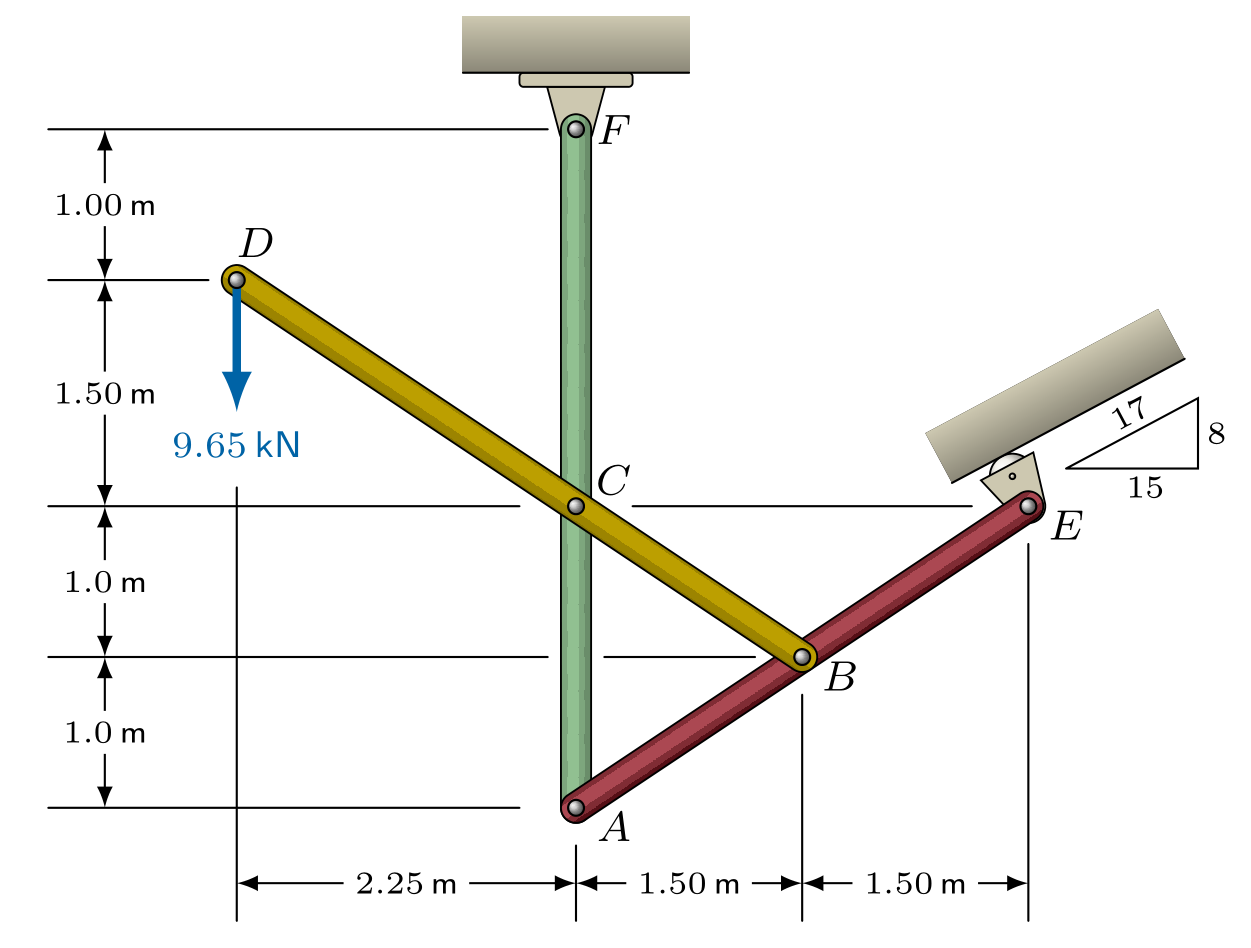
\includegraphics[width=1.25\linewidth]{includes/cf.png}\par\noindent
% 	Determine the magnitude of the reactions at all connections and the roller when a 9.65 kN force is applied vertically downwards at $D$.\vspace{0.5cm}
% }
% \parm
LMSes don't offer question types that mark multiple parts for each question although it is a much requested functionality (particularly, it seems, on Canvas).\sidenote{https://community.canvaslms.com/thread/5891}\sidenote{https://app-community.canvaslms.com/ideas/8172-multiple-numerical-blanks}\sidenote{https://community.canvaslms.com/thread/30523-multiple-part-formula-question}

\parm
Moodle\sidenote{https://moodle.org} is a popular open-source LMS that offers an impressive list of question-types\sidenote{https://docs.moodle.org/37/en/Question\_types} but no mention of a random-input multiple-part question type. However, there is a Moodle plug-in (initiated in 2010 by Hon Wai Lau\sidenote{https://www.linkedin.com/in/hon-wai-lau-97508182}) that provides the required functionality.\sidenote{https://github.com/jmvedrine/moodle-qtype\_formulas} I have built a handful of sample questions\sidenote{{\scriptsize http://eduk8r.org/moodle/mod/quiz/view.php?id=24} \\User: learner, Password: Le@rner1} using this plug-in and consider it to be a realistic solution for those institutions that adopt Moodle as their LMS.
\newpage
In 2008, I wrote a simple testing system,\sidenote{http://qwizm.org} that provides a limited set of quizzes or assignments comprised of multiple-part questions and used them for assignments in introductory engineering courses.
\parm
This proposed capstone project will be a refactorization of this early project, using more modern web technologies and with the aim of streamlining question creation. A second objective is to establish a cleaner codebase for Qwizm that could be generated by a future desktop application.

\section{\Large Scope}

I had initially hoped to create the final desktop application project as my capstone but have concerns about completing that project within the allotted timeframe. I have been informed by Jose Ramirez during a Zoom conversation that the final desktop application would be beyond the scope of a capstone project. I do feel that the work proposed here would be equivalent to 2-3 courses' assignments and projects.

\section{\Large Similar Work}
Apart from the Moodle plugin mentioned above and linked to here again,\sidenote{https://github.com/jmvedrine/moodle-qtype\_formulas} I am not aware of any multiple-part numerical answer quizzes that fully satisfy the same requirements. They may, of course, exist.
\parm
In more detail, the Moodle Formulas question type plugin allows creation of questions with multiple-part answers, although within the heavy structure of an LMS. It does not directly provide feedback for each question part as the answer is added --- although, by submitting the full question for marking after each answer part is entered, the student can see whether or not they have been successful (this requires that the Moodle question be set to allow unlimited attempts). It does not allow for input values to be super-imposed on the static question diagram, nor for a student to practise the questions with different inputs (by using a different ID number).

\section{\Large Novelty}
I am not aware of any directly similar work.

\section{\Large Rubric}
I will feel that my capstone has been successful if either, or both, of the following results:
\begin{itemize}
	\item Question creation will be streamlined, enabling me to more rapidly develop a problem set for a complete course in engineering statics. Qwizm, as it currently exists, is unwieldy and more a proof of concept than a usable tool.
	\item An efficient codebase that can be used as the basis for code generation by a future desktop application.
\end{itemize}

\section{\Large Technologies Used}
\begin{description}
	\item[Technology \#1 JavaScript/ECMAScript 6:] Used to create reproducible pseudo-random numbers for question input values, for checking whether submitted answers are correct or incorrect, to store submitted values and marks earned in local storage and to control the visibility of questions or the summary page in what will be a single page application.
	\item[Technology \#2 CSS3:] Used to make the site responsive, using media queries to control layout on different devices. A mobile-first pattern will be followed although it is expected that Qwizm will be more useful on a tablet or computer.
	\item[Technology \#3 HTML5:] Used for more semantic tags and for local storage to maintain the state of quizzes between browser sessions and to recognise whether a user has previously accessed a particular quiz.
\end{description}
% Note: I have decided not to use ReactJS for this project, primarily because the build process produces a complex minimised project that is not much help when it comes to having a codebase for a future desktop application to generate. I shall investigate using simple web components, built from scratch.

\section{\Large Tentative Schedule and Milestones}
\begin{description}
	\item [Milestone #1 (Week 1)] Develop login: Check whether a quiz object for this quiz exists in local storage. If so, directly log user in and load quiz from local storage into memory. Othewise, create the quiz object containing student name and ID. The user will have an option to clear the quiz object, and all work currently completed, necessitating a new login. This provides the student with the option to enter a fictitious ID number to get different values for question inputs.
	\item[Milestone #2 (Week 2)] Responsive Design: Write the CSS to make the site responsive for different screen sizes.
	\item[Milestone #3 (Week 4)] Refactor Utility Classes: This will involve rewriting functions such as the one that marks the answers correct or incorrect. Arguments will be added to allow the question builder, i.e. the teacher or instructor, to set different tolerances for correct marks, ranging from exact, e.g. 3.40 is correct, 3.4 is not when requiring three significant digits, to an allowable relative or absolute percentage error. An encrypt/decrypt function will be investigated to see if it is practical to encrypt values in variables, thereby preventing students from using developer tools in the browser to view correct answers.
	\item[Milestone #4a (Week 5)] Design JSON objects for questions: Question specifics will be stored in a JSON object, with key-value pairs for: numerical identifier; named input variables determined by low, high and incremental values, question statement including input variables (actual numbers will be written at runtime); equations to determine required answers based upon input variables; path to static image; values to be superimposed on the static image, together with their location; question parts with answers in the form of a single variable, accuracy required and marks assigned to each question part.
	\item[Milestone #4b (Week 5)] Design the JSON object for quiz: Quiz specifics will be stored in a JSON object with key-value pairs for: course; topic; due date; list of questions.
	\item[Milestone #5 (Week 9)] Process quiz and question objects: Write the code that processes the quiz and included questions, building the whole quiz functionality.
	\item[Milestone #6 (Week 10)] Build a sample quiz: Produce a quiz, comprised of questions involving relatively straightforward algebra and trigonometry so that the project can be tested by someone not having a background in engineering. This will also serve as a math review for students at the beginning of their engineering program.
\end{description}



\section{\Large Project Description}\label{sec:background}

Despite its limitations, the original Qwizm has proved to be effective both as an assessment tool and as a learning tool. It continues to be used by the instructor who has taken over teaching my courses following my retirement from teaching.
% The refactoring proposed here is the first part of a larger project to build a desktop application that will enable instructors with no programming knowledge to develop their own questions and to combine questions to make quizzes.
\parm
Currently, question development is laborious and requires a knowledge of JavaScript, knowledge that instructors, in general, do not possess. A complex question can take several hours to produce and this lengthy development time is in large part responsible for Qwizm remaining positioned somewhere between a proof of concept and a complete course assessment resource.

\parm
There are several motivations for this proposed refactoring of Qwizm: to speed up development time for new questions and quizzes, thereby encouraging further development of question banks; and to make the application more user-friendly from a student perspective, providing a responsive site that they may conveniently access on different devices and that retains previously entered values between browser sessions.
\parm
The primary motivation, though, is to realise an efficient codebase that could be generated by a future desktop application. This application would enable instructors to package and distribute a collection of multiple-part numerical questions as a single minimised html file.  No programming knowledge would be required though the ability to build a formula, as in a standard spreadsheet, would be necessary.
\parm
The screenshot below is a typical example of a Qwizm question from a water resources course. (A 'live' version can be seen at  \href{http://qwizm.org/fluids/08HW/quizzes/HWSet01/index.html}{http://qwizm.org/fluids/08HW/quizzes/HWSet01/index.html}.) Pipe characteristics and elevation difference between the two tank surfaces are randomized so that students get different input values to work with.
\parb
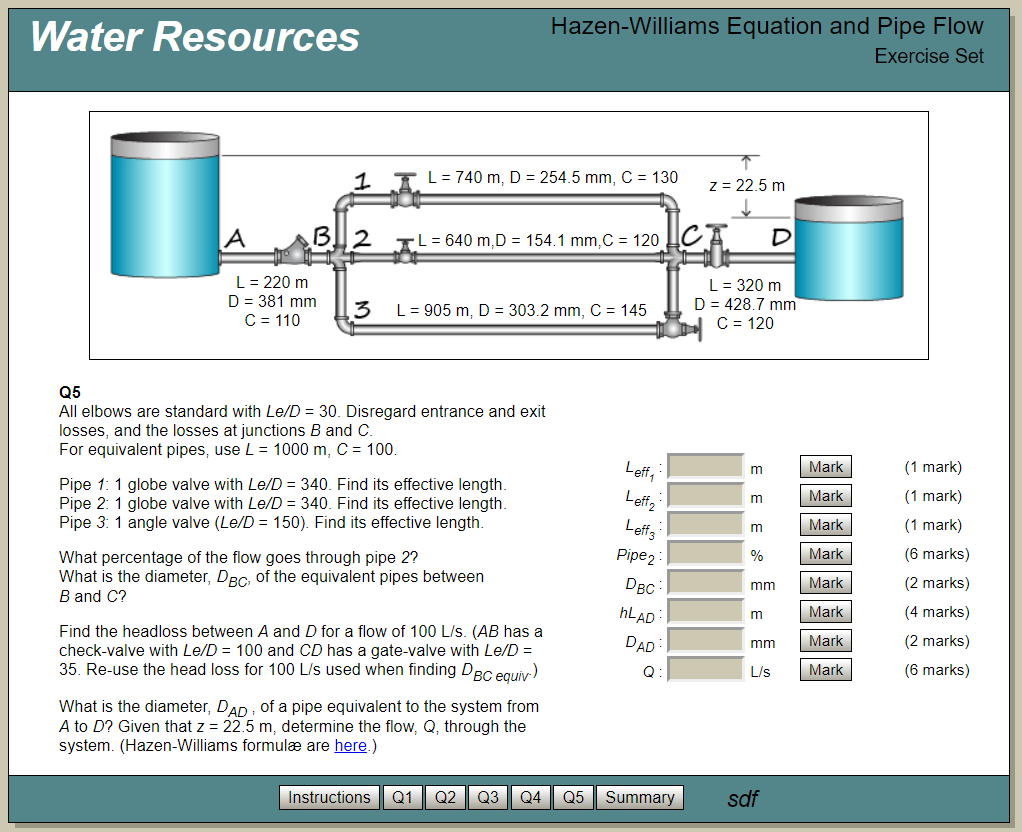
\includegraphics[width=1\linewidth]{includes/hw.png}
\parb
\newpage
This is a complex question and would take about 40 minutes to go through in class. Without the feedback from the question parts it would not be realistic to expect a student to arrive at the correct final answer. In this case, it is only the final answer that we are interested in but the earlier parts provide guidance towards this final value.
\parb
The question below, from an engineering statics course and not implemented on Qwizm, asks for several different answers:
\cmini{
\footnotesize
There is a frictionless roller at $E$ and pinned connections at $A$, $B$, $C$ and $F$.
\parb
\begin{centering}
	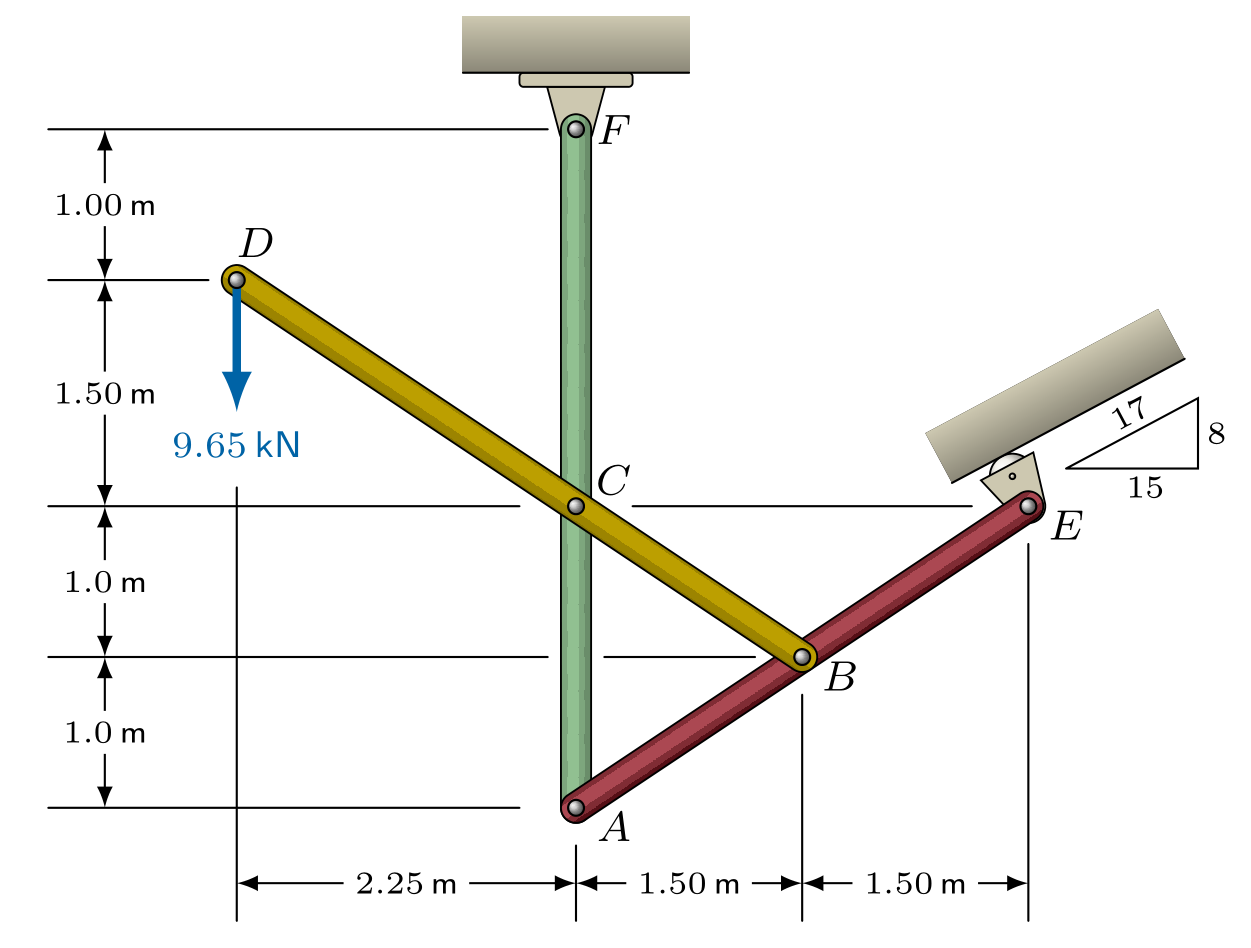
\includegraphics[width=0.8\linewidth]{includes/cf.png}
\end{centering}

Determine the magnitude of the reactions at all connections and the roller when a 9.65 kN force is applied vertically downwards at $D$.
}
\parb
Such a question, with randomized inputs for lengths and the applied force, is an excellent candidate for Qwizm.
\parb
Note: Both the above figures were created by myself.
\parb
I accept the reality that there is no way to guarantee that all students work independently on assignments. Individualized question inputs do not solve the problem of unwarranted collaboration but they do help with learning. Even when the next step in a problem has been discussed in a group, each student does, at least, perform their own calculations --- and to write out their own solution which is submitted together with Qwizm's printed summary sheet.
\parm
Although I have used these Qwizms almost exclusively for assignments that count towards a final course grade, some students choose to re-do them, possibly with a different ID number to generate different inputs, as review before mid-term and final exams. With a more comprehensive question library, they could also be used as an alternative to 'static' in-class examples or exercises.
\parm


For many instructors, the attraction of online testing is the associated reduction in time spent marking student work. This comes with some cost; not actually seeing student work until exam-time can be a time-saver for instructors but successful steering of students towards a logical and professional presentation of material is more difficult to assess.
\parm
Qwizm, with its instant feedback and traditional paper-based submission, does have some advantages:
\begin{enumerate}
	\item The instant feedback from question parts encourages students to persist until they have the right process and the correct answer for that part before continuing. Indeed, students realise that there is little point in continuing since future results usually depend on the successful completion of earlier steps.
	\parm
Prior experience with existing commercial LMS assignments had less successful outcomes as far as student motivation was concerned: students would complete an assignment online, submit it for marking, find they had scored, say, 70\% but felt frustrated by having to retake the whole assignment, with fresh inputs to questions they had already completed successfully, to improve their mark. In contrast, Qwizm, with its continual feedback, encourages students to persist towards completion; it is common for students to get 100\% on Qwizm assignments.
\parm
(Although completion of these assignments can be quite lengthy, in my courses they only count for 10\% of the total course mark; that is substantial effort for a somewhat minor return in marks but students recognise that these are a good way to learn material and the time spent will serve them well at exam time.)
\parm
Other attempts at online assessment using offerings from textbook publishers were also a source of frustration; for the text that we tried this with, answers were frequently incorrect with no way for the instructor to correct them, most questions did not have randomized inputs but were simply the same as questions from the text, and students wondered what they were obtaining in exchange for their required subscription to the publisher's testing site.
	\item Compared to traditional paper submissions, the marking burden on the instructor is dramatically reduced: marks are already calculated, ready for entry into an LMS or spreadsheet, and the written work can be quickly viewed for completeness, professionalism, etc. It is not unreasonable to process a student assignment in less than one minute.
\end{enumerate}



%
% \bibliography{capstoneProposalDaveMorgan}
% \bibliographystyle{plainnat}



\end{document}
